\documentclass[12pt, letterpaper]{article}
\usepackage[a4paper,left=3cm,right=2cm,top=2.5cm,bottom=2.5cm]{geometry}

\usepackage[utf8]{inputenc}
\usepackage{graphicx}
\graphicspath{ {images/} }
\usepackage{amsmath,bm}
\usepackage{listings}
\usepackage{float}
\usepackage{pdfpages}
\usepackage{siunitx}
\usepackage{subfig}


\title{4TN4 Assignment 5}
\author{Adam Bujak (400113347)}
\date{March 13, 2022}

\begin{document}

\maketitle

\section{Theory}

\subsection{Harris Corner Detection}

\subsection{Scale selection, LoG}

The LoG of an image is represented by the formula 

\[LoG(x,y) = - \frac{1}{\pi\sigma^4}\cdot (1-\frac{x^2 + y^2}{2\sigma^2})\cdot e^{-\frac{x^2+y^2}{2\sigma^2}}\]

To achieve the maximum response, the zeros of the Laplacian must be aligned with the edges of the circle, therefore:

\[0 = - \frac{1}{\pi\sigma^4}\cdot (1-\frac{x^2 + y^2}{2\sigma^2})\cdot e^{-\frac{x^2+y^2}{2\sigma^2}}\]

and since 

\[x^2 + y^2 = r^2\]


\[0 = (1-\frac{r^2}{2\sigma^2})\cdot e^{-\frac{r^2}{2\sigma^2}}\]

\[0 = 1-\frac{r^2}{2\sigma^2}\]
\[1 = \frac{r^2}{2\sigma^2}\]
\[\sigma = \pm\sqrt{\frac{r^2}{2}}\]
\[\sigma = \frac{r}{\sqrt{2}}\]

\subsection{RANSAC}

$p$ is the probability that at least one of the sets does not include an outlier. Therefore $1-p$ is the probability every set includes outliers. $u$ is the probability of any point being an inlier, therefore:

\[1-p = (1-u^m)^N\]

\[N = \frac{log(1-p)}{log(1-u^m} \]

\[N = \frac{log(1-0.99)}{log(1-0.7^2)} \]

\[N = 6.83 \]
\[N \simeq 7 \]

\section{Implementation}

\section{Implementation}

\subsection{Change point of view}
\begin{figure}[H]
    \centering
    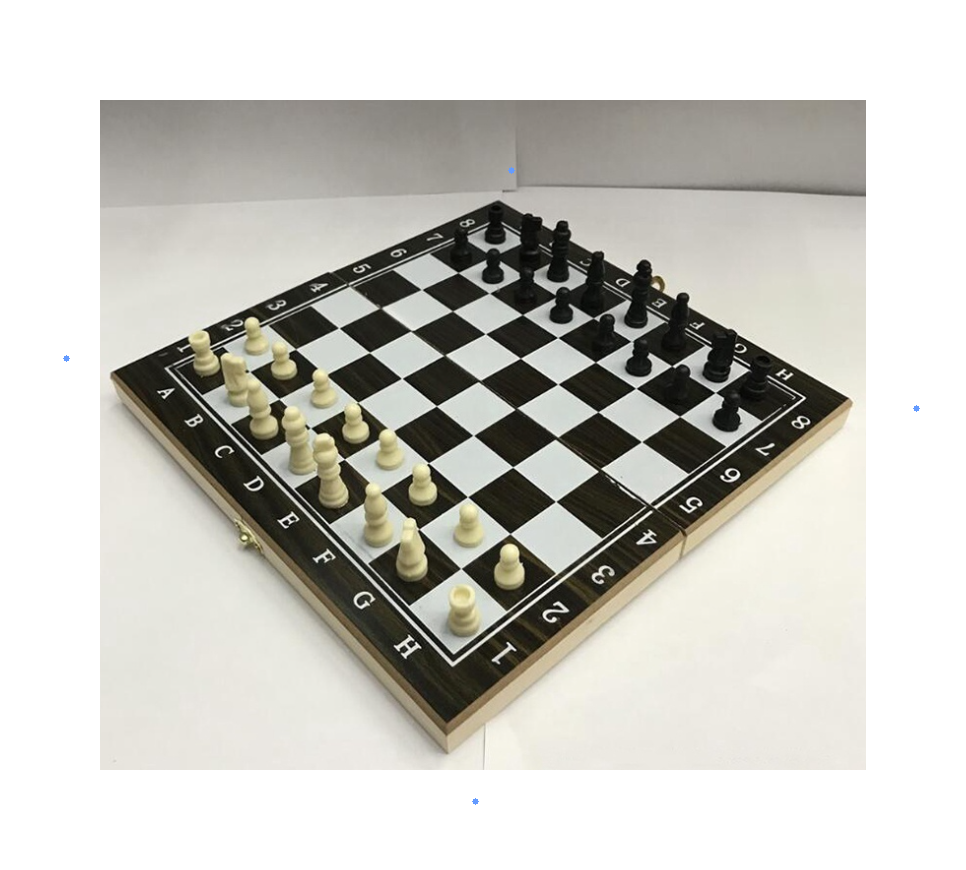
\includegraphics[width=\textwidth]{chesspts.png}
    \caption{Points selected for transformation}
\end{figure}

\begin{figure}[H]
    \centering
    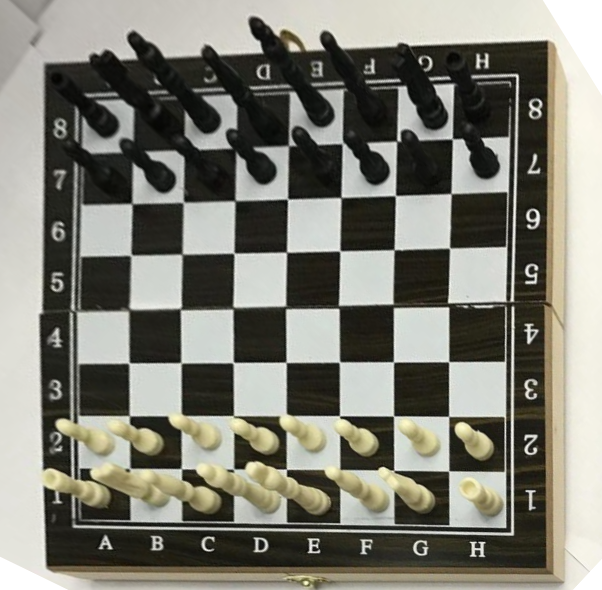
\includegraphics[width=\textwidth]{new_chess.png}
    \caption{Transformed image}
\end{figure}

\begin{figure}[H]
    \centering
    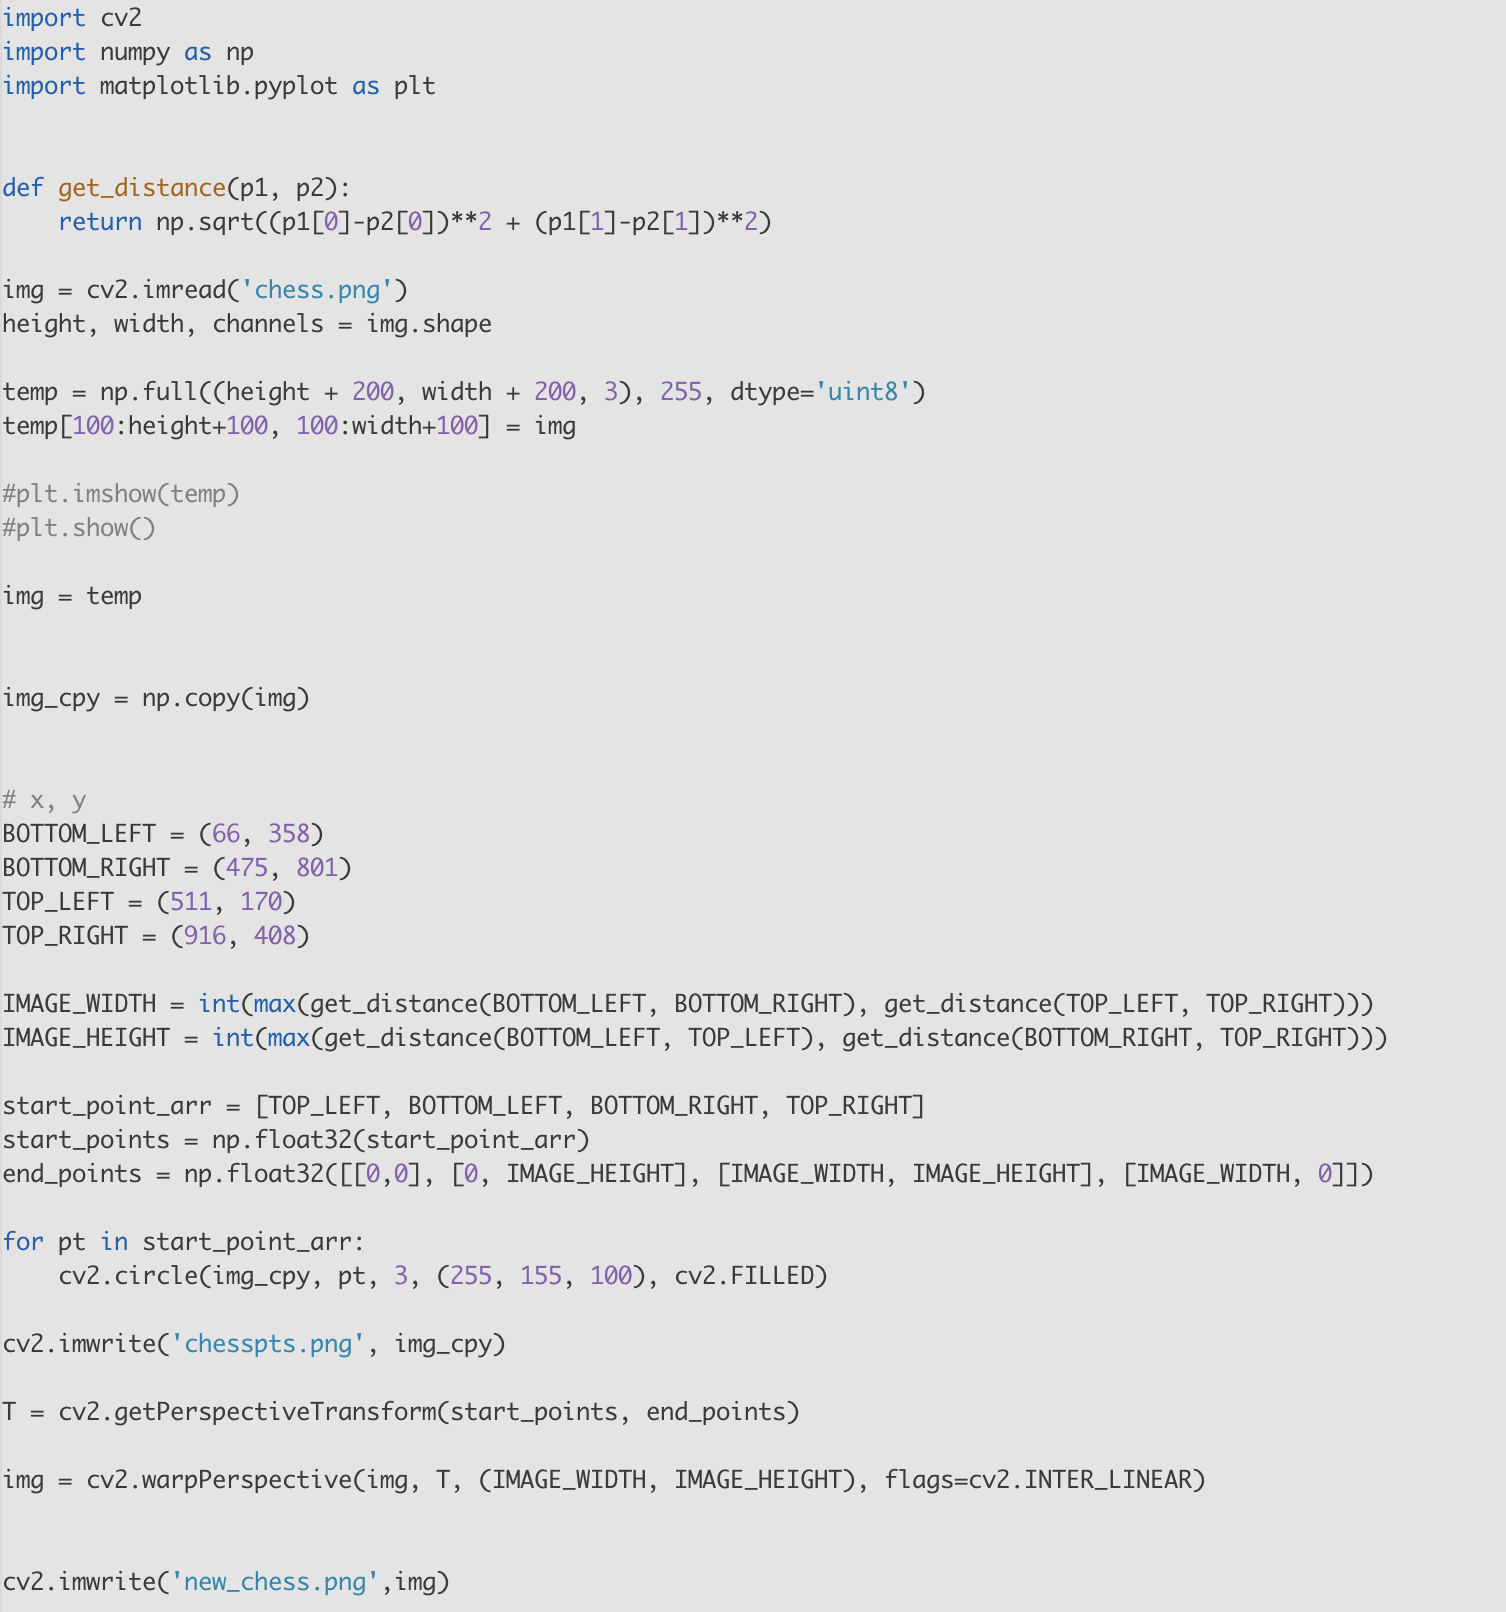
\includegraphics[width=\textwidth]{q1.png}
    \caption{Code used to transform image}
\end{figure}

I needed 4 points to execute this transformation.

\subsection{Visualize Matched points}

Using SIFT:

\begin{figure}[H]
    \centering
    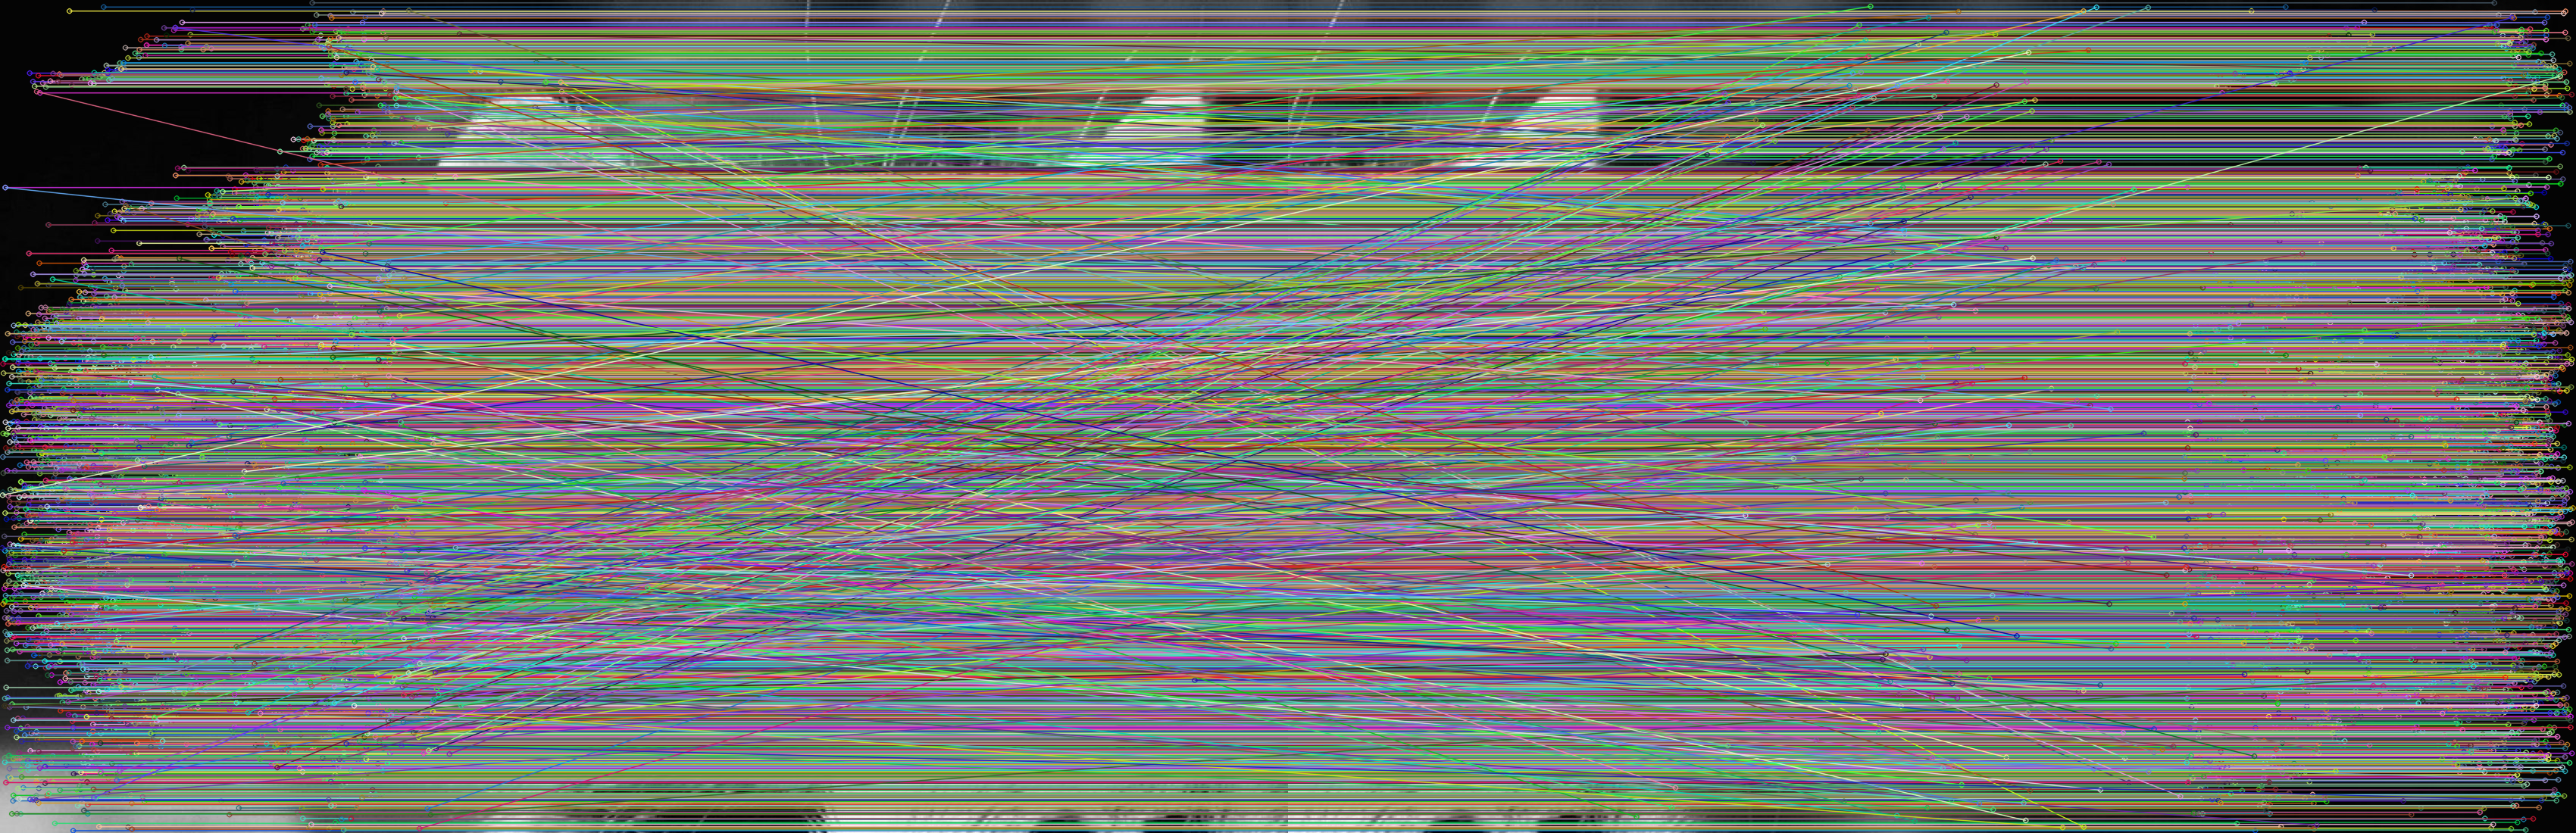
\includegraphics[width=\textwidth]{image_1_matches.png}
    \caption{Matched images}
\end{figure}

\begin{figure}[H]
    \centering
    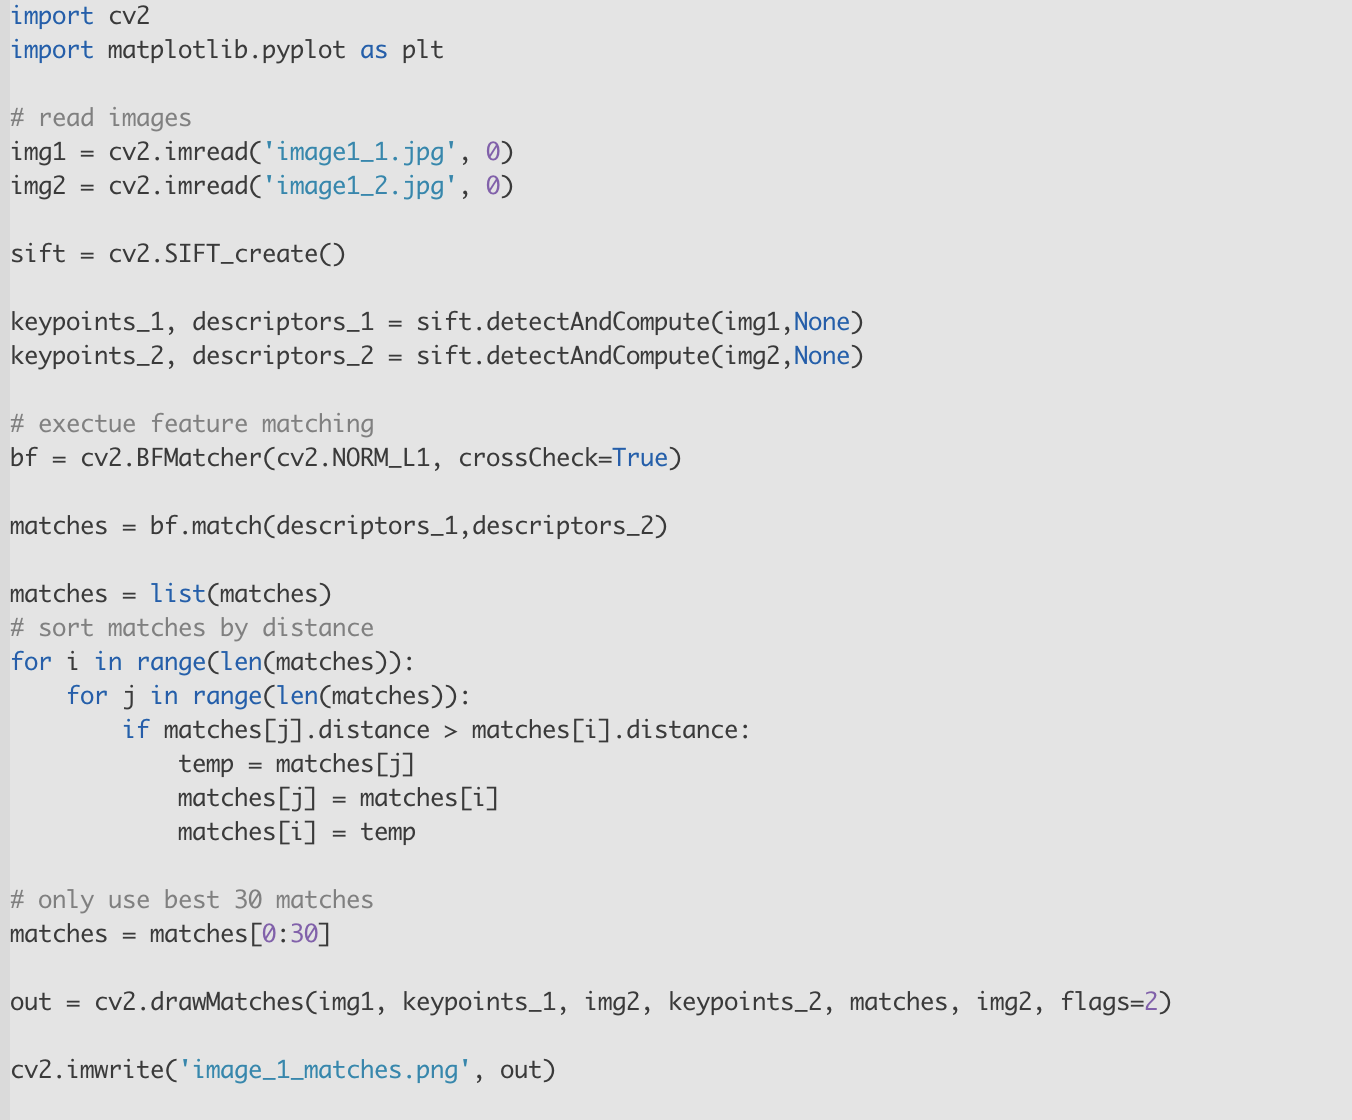
\includegraphics[width=\textwidth]{q2.png}
    \caption{Code used to match features}
\end{figure}

\subsection{Solving a puzzle}

\begin{figure}[H]
    \centering
    
\includegraphics[width=\textwidth]{out3.png}
    \caption{Solved Puzzle}
\end{figure}

\begin{figure}[H]
    \centering
    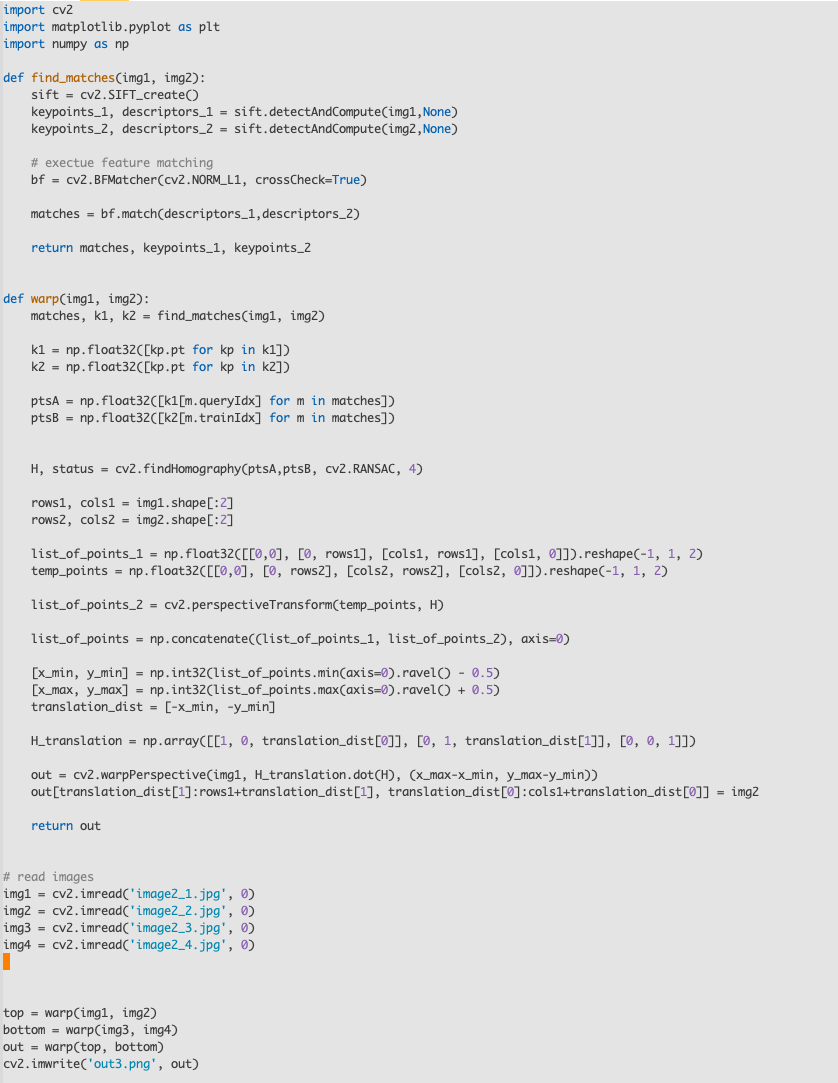
\includegraphics[width=\textwidth]{q3.png}
    \caption{Code used to merge images}
\end{figure}


\end{document}
)}]
